% !TeX program = xelatex
\documentclass[UTF8,11pt,a4paper,linespread=1]{ctexart}
\usepackage[margin=26mm]{geometry}
\usepackage{amsmath,amssymb,bm}
\usepackage{setspace}
\setstretch{1.35}
\usepackage{pgfplots,subcaption}
\pgfplotsset{compat=1.18}
\captionsetup{subrefformat=parens}
\usepackage[unicode,colorlinks=true,linkcolor=teal]{hyperref}

\begin{document}
\section*{同一坐标范围下比较两条曲线}
\begin{figure}[htbp]
\centering
\begin{subfigure}[t]{.47\linewidth}
  \centering
  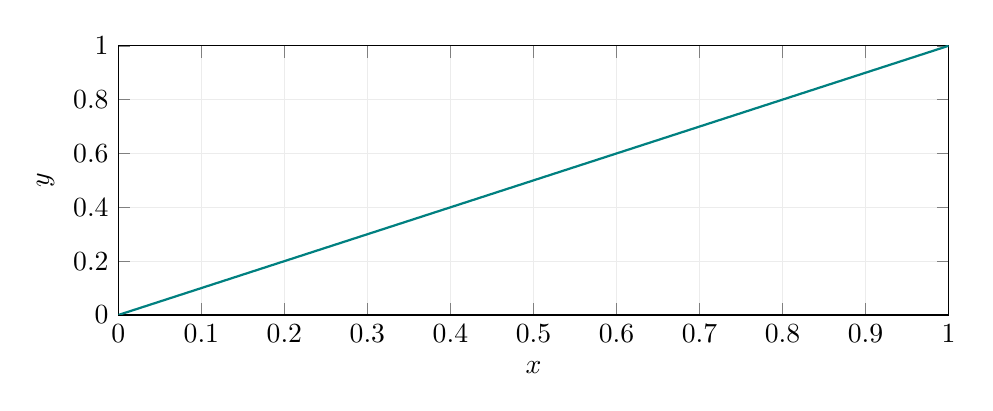
\begin{tikzpicture}
  \begin{axis}[width=\linewidth,height=5cm,
    xmin=0,xmax=1,ymin=0,ymax=1,
    xlabel={$x$},ylabel={$y$},grid=major,grid style={gray!15}]
    \addplot[teal,thick,domain=0:1,samples=81]{x};
  \end{axis}
  \end{tikzpicture}
  \caption{线性关系}\label{fig:linear}
\end{subfigure}\hfill
\begin{subfigure}[t]{.47\linewidth}
  \centering
  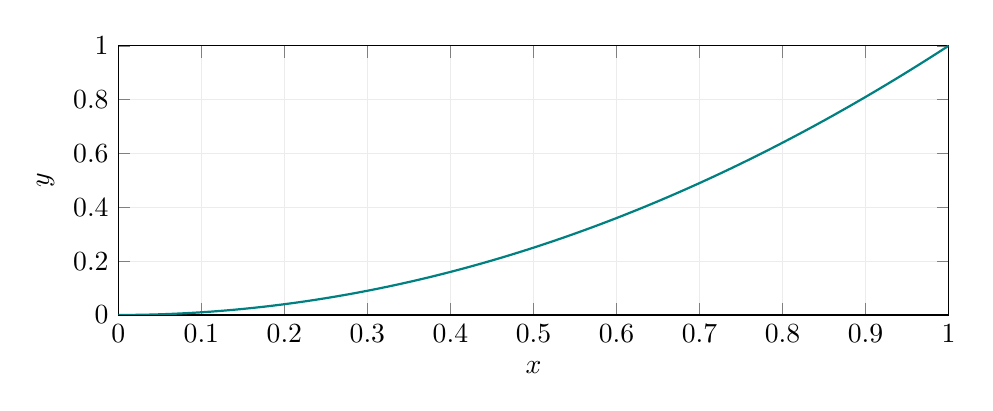
\begin{tikzpicture}
  \begin{axis}[width=\linewidth,height=5cm,
    xmin=0,xmax=1,ymin=0,ymax=1,
    xlabel={$x$},ylabel={$y$},grid=major,grid style={gray!15}]
    \addplot[teal,thick,domain=0:1,samples=81]{x^2};
  \end{axis}
  \end{tikzpicture}
  \caption{二次关系}\label{fig:quadratic}
\end{subfigure}
\caption{相同坐标尺度下的函数对比}\label{fig:compare}
\end{figure}
图~\ref{fig:compare} 中，子图~\subref{fig:linear} 与
子图~\subref{fig:quadratic} 使用相同的横纵坐标范围。

\end{document}
